\chapter{Literature study}
\label{chap:literature}

This chapter presents an overview of literature that is related to this work. The first section will summarize the mobile application architectures that are currently used to create cross-platform solutions. In the second section, a generic software evaluation and selection methodology will be explored. In the third and last section, a number of techniques for multi-criteria decision making are studied, together with their strengths and weaknesses.

\section{Mobile application architectures}

Building cross-platform solutions starts at the architectural level. This section will discuss the architectures that are currently used with mobile applications or apps for short \cite{Friese}. Mobile architectures comprise of three key elements: 

\begin{itemize}
    \item The \emph{mobile device} is the piece of hardware that runs the actual application. This is the place where the architectures will differ the most.
    \item The \emph{backend} is a service, provided by one or more servers that store all the application data. This could be a web service, ERP software like SAP, a CRM system like Salesforce, etc. or it could be a combination of such services.
    \item The \emph{mobile hub} or\emph{mobile orchestrator} is a server that acts as a mediator between the mobile device and the backend. It is put in place for multiple reasons: it exposes a uniform interface to the mobile device (and hides external API changes), prevents distributed denial-of-service (DDoS) attacks from the large number of mobile devices connecting to the backend, can cache information to reduce the load on the backend, can inject services like advertising into the application, etc.
\end{itemize}

The architecture of the native application is discussed first and is used as a reference architecture. For each of these architecture, a number of aspects will be highlighted: performance, look \& feel, platform access, programming languages, development cost and distribution.

\subsection{Native application}

A native application is an application that is specifically designed to run on a particular platform. It is the default approach to develop applications for mobile devices and is therefore considered the reference architecture in this section. It is illustrated in \fref{fig:native}. 

\begin{figure}[h]
    \begin{center}
        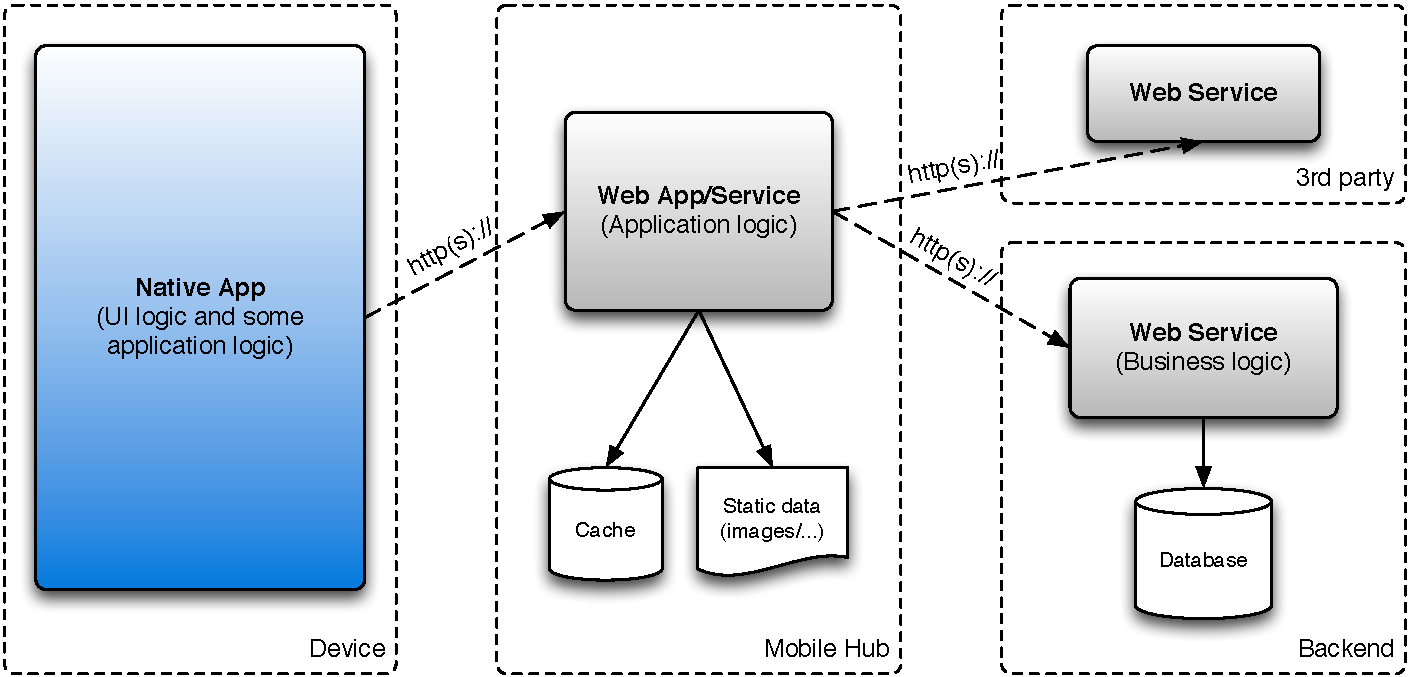
\includegraphics[width=\textwidth]{figs/native.pdf}
        \caption{Architecture of a native application. Based on \cite{Friese}}
        \label{fig:native}
    \end{center}
\end{figure}

Native applications are developed with the supplied software development kit (SDK). That SDK uses a particular programming language that developers will have to learn together with the features of the SDK. In return they will get full access to the platform and its features. As a result, the best performance can be achieved with this kind of application.

The SDK also provides a large number of user interface elements that developers can use to create a rich user interface that is consistent with the look \& feel of the platform. This is called native look \& feel. Native apps are typically distributed through an online marketplace like the App Store for iOS applications or Google Play for Android applications. 

The development cost of native applications is high because developers need to be familiar with multiple SDKs and the application has to be developed separately for every platform that has to be supported.

\subsection{Mobile web application}

Mobile web applications are websites that are optimized for mobile browsers. Since every platform comes with a browser, this is the easiest way to get an application running on all platforms. An overview of this architecture is depicted in \fref{fig:web}. Mobile web applications are built with HTML (content), JavaScript (behaviour) and CSS (styling, are viewed in the browser and are distributed on the Internet with a URL but they cannot be installed on the device. A workarounds using Web Clips \cite{Safari:webclips} is available on iOS and on Android, bookmarks can be placed on the home screen. 

\begin{figure}[h]
    \begin{center}
        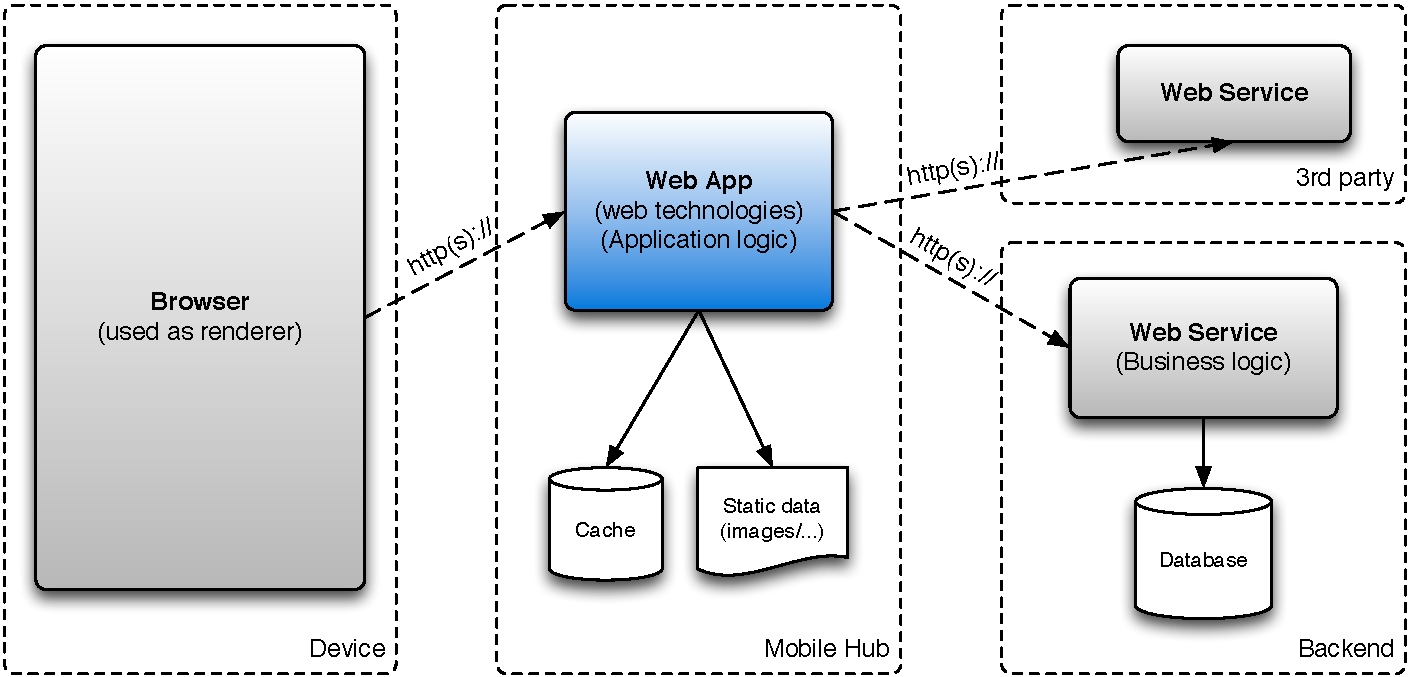
\includegraphics[width=\textwidth]{figs/web.pdf}
        \caption{Architecture of a mobile web application. Based on \cite{Friese}}
        \label{fig:web}
    \end{center}
\end{figure}

Mobile web applications are not nearly as powerful as native applications because the web is currently not a first-class platform. Many mobile web browsers lack support for particular HTML5 features. These defects are listed on websites like ``Can I use...''\footnote{\url{http://caniuse.com}} and ``Mobile HTML5''\footnote{\url{http://mobilehtml5.org}}. Developers should constantly check whether a certain feature is available. In some cases, the missing feature can be \emph{polyfilled}. This term polyfill is inspired by the famous wall filler ``Polyfilla'' and is used for additional pieces of code that provide the missing HTML5 functionality. However, no polyfill can provide access to the underpinning hardware. Most mobile web applications also require an internet connection because the application is not cached in the browser. 

Mobile web applications cannot make use of the native user interface elements. Because of this limitation, it is hard to provide a native look \& feel. There are a number of project that try to mimic the native user interface elements with HTML templates and custom styles. However, the styling is quite complex and additional behaviour is added to animate these elements, which is disadvantageous for the performance. On the other hand, some people believe that the web is a platform of its own because it satisfies the ``one size that fits all'' philosophy. Therefore, it is entitled to its own look \& feel \cite{Mahemoff:2011}.

The development cost of mobile web applications is low because it does not require additional skills (web development is often already in the skill portfolio) and the application has to be developed only once and can serve all platforms. 

\subsection{Hybrid application}

A Hybrid application is the combination of a native application and a mobile web application. The actual application is a mobile web application that is embedded in a native application and made visible through a WebView\footnote{A WebView is a native user interface element that displays web content inside applications.}. The native shell offers a JavaScript bridge to the web application, allowing the web application to access to the system. Because hybrid applications and wrapped in a native shell, they can be distributed through (official) marketplaces. The architecture is visualized in \fref{fig:hybrid}.

\begin{figure}[h]
    \begin{center}
        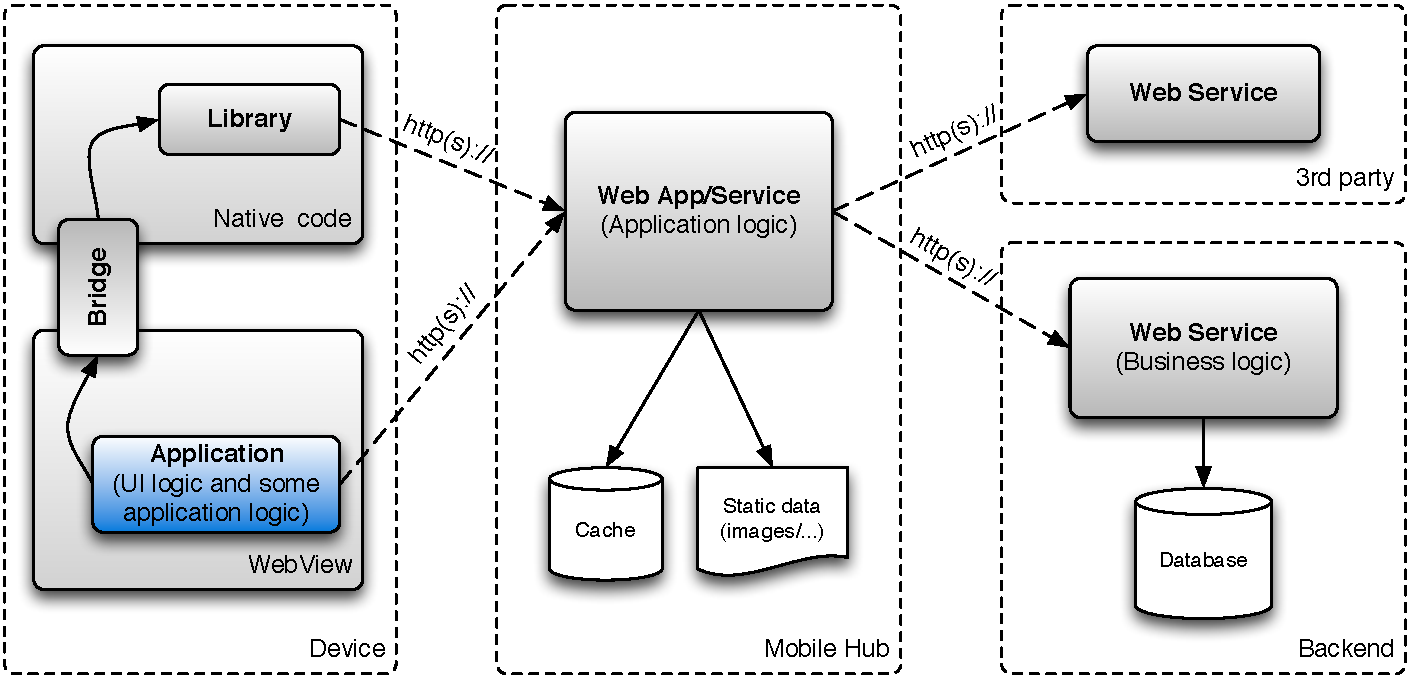
\includegraphics[width=\textwidth]{figs/hybrid.pdf}
        \caption{Architecture of a hybrid application. Based on \cite{Friese}}
        \label{fig:hybrid}
    \end{center}
\end{figure}

Because of the nature of the application, the performance is be similar to web applications. Unlike mobile web applications, hybrid applications are more flexible because they allow better integration with the device through the JavaScript bridge. This way, missing features can be implemented natively and accessed through said bridge. Another consequence of its nature is that hybrid applications do not use the native user interface elements and cannot provide the native look \& feel. 

The development cost of hybrid applications is similar to that of mobile web applications because wrapping web applications does not require any knowledge of the native SDK's. 

\subsection{Interpreted application}

Interpreted or runtime applications try to solve the platform differences by introducing an intermediary programming language. Instructions from that language are translated to native instructions at runtime. Interpreted applications are similar to Java applications on the desktop. From the outside, interpreted applications look just like native applications and can be distributed through online marketplaces. An interpreter or runtime is built right into the application, which increases the installation size of the application. This could be disadvantageous on low-end smartphones with limited storage capabilities. The architecture of an interpreted application is demonstrated in \fref{fig:interpreted}.

\begin{figure}[h]
    \begin{center}
        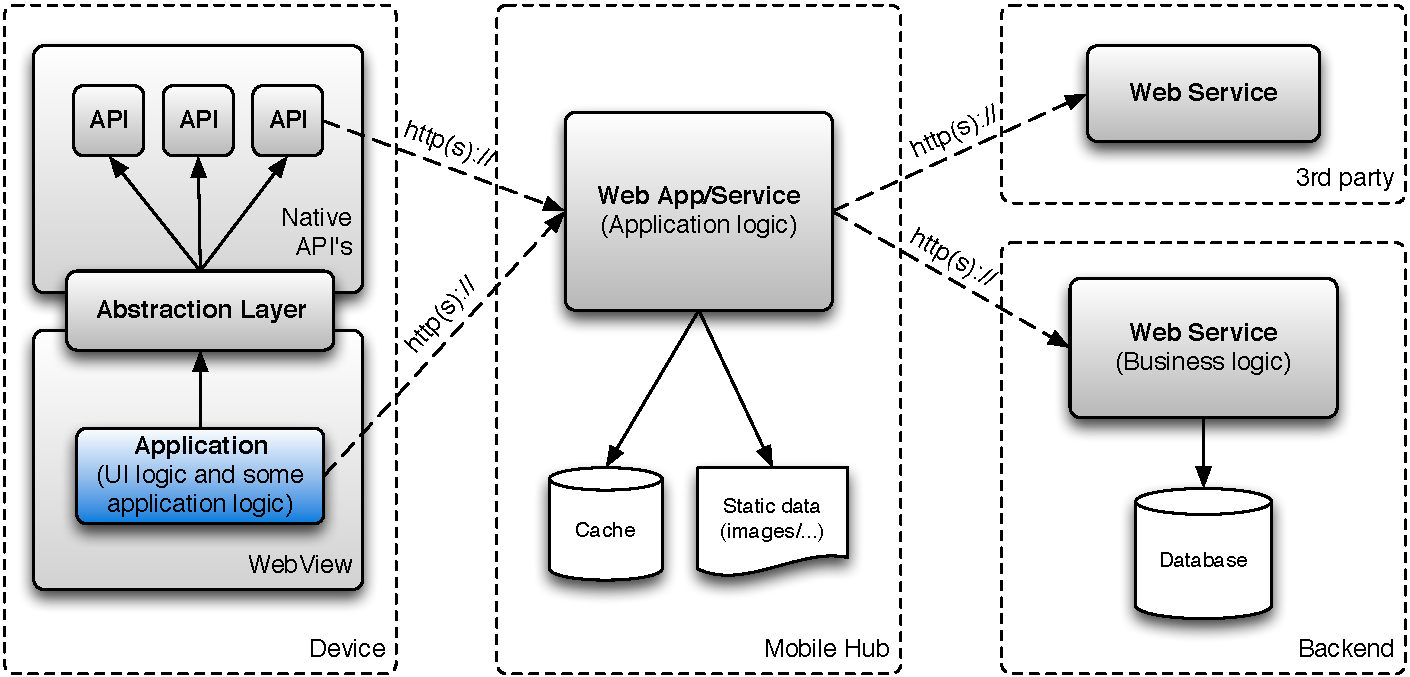
\includegraphics[width=\textwidth]{figs/interpreted.pdf}
        \caption{Architecture of an interpreted or runtime application. Based on \cite{Friese}}
        \label{fig:interpreted}
    \end{center}
\end{figure}

The performance of an interpreted application strongly depends on the interpreter itself and the interpreted programming language. In general, the performance is better than the performance of web applications but it is not as good as the performance of native applications. Because of the nature of interpreted applications, the native user interface elements can be used to provide a native look \& feel.

The development cost of interpreted applications is a higher than the cost of mobile web applications but lower than the cost of native applications. Developers need to be familiar with the SDK of the cross-platform tool but the application has to be developed only once and can be run on all supported platforms.

\subsection{Cross-compiled application}

In contrast to interpreted applications, instructions of cross-compiled are translated at compile time. The resulting application is not noticeably different from a native application because no runtime has to be included. This architecture is presented in \fref{fig:crosscompiled}. 

\begin{figure}[h]
    \begin{center}
        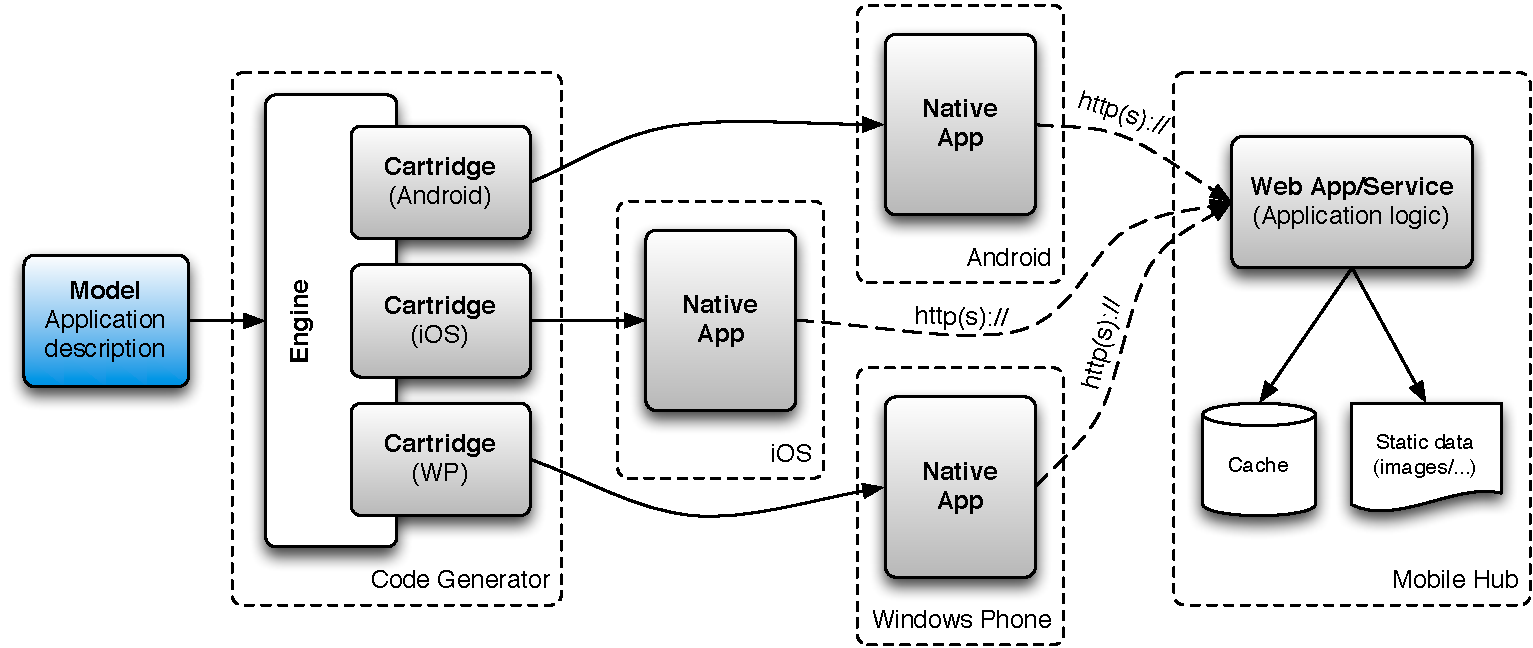
\includegraphics[width=\textwidth]{figs/crosscompiled.pdf}
        \caption{Architecture of a cross-compiled application. Based on \cite{Friese}}
        \label{fig:crosscompiled}
    \end{center}
\end{figure} 

Because the application only exists of machine code, the performance of cross-compiled applications is nearly identical to the performance of native applications. Cross-compiled applications can make use of the native user interface elements and consequently provide the native look \&feel. However, this sometimes requires custom bindings for each platform, increasing the amount of code that has to be written. 

The development costs of cross-compiled applications is similar to the costs of interpreted applications. Developers still need to be familiar with the SDK of the cross-platform tool but the application has to be developed only once and can be run on all supported platforms. Also, not all code can be reused in cross-compiled applications, which raises the development costs a little more.

\subsection*{Comparison of mobile architectures}

To conclude this section, the discussed architectures are compared side by side. The results are shown in \tref{tab:architectures}. Every architecture has both strengths and weaknesses. Therefore, the architecture must be chosen carefully, taking the client's wishes into account. 

\begin{table}[h]
    \begin{center}
        \begin{tabular}{lccccc}
            \hline
                            & Native      & Web         & Hybrid      & Interpreted & Cross-compiled\\
            \hline
            Performance     & high        & low         & low         & average     & high          \\
            Hardware access & \checkmark  & partial     & \checkmark  & \checkmark  & \checkmark    \\
            Look \& Feel    & native      & non-native  & non-native  & native      & native        \\
            Distribution    & store       & URL         & store       & store       & store         \\
            Cost            & high        & low         & low         & moderate    & moderate      \\
            \hline
        \end{tabular}
		\caption{
			Summary of cross platform mobile application development strategies.
		}
		\label{tab:architectures}
    \end{center}
\end{table}

\section{Software evaluation methodology}
\label{sec:sw-selection}

Based on their literature review \cite{Jadhav:2009}, the authors have proposed a generic, six-stage methodology for the selection of software packages \cite{Jadhav:2011}.

\begin{enumerate}
    \item \textbf{Define selection criteria.} In the first stage, the evaluator defines the essential requirements for the software. If a certain software package does not meet a selection criterion, it is not a considered to be a suitable candidate and it should not be considered for further evaluation. 
    \item \textbf{Identify potential candidates.} During the next step, the evaluator searches for potential candidates. This step will result in a list of potential candidates.
    \item \textbf{List selected alternatives.} In this step, the evaluator will use the requirements from stagdate 1 to filter the list obtained from the previous stage. 
    \item \textbf{Define evaluation criteria.} In this stage, the evaluator has to define the evaluation criteria, arrange them in a hierarchy and define the value scales for each criterion. 
    \item \textbf{Evaluate selected alternatives.} During this phase, the evaluator will make a detailed comparison of the alternatives using the criteria obtained from the previous stage. A methodology like AHP can be used in this stage.
    \item \textbf{Select the most suitable alternative.} In this final step, all alternatives are ranked using the comparison results from the previous stage. Now, the best alternative can be chosen from the list of candidates. In general, a number of software packages will be taken into consideration and a selection will be made after additional steps (like for instance a cost-benefit analysis and/or contract negotiations with the vendor). 
\end{enumerate}

In the original paper \cite{Jadhav:2009}, the authors also suggest to include an additional evaluation stage after the selected packages has been implemented and integrated. During that stage, one should verify that the selected package does indeed meet the requirements.


\section{Multi-Criteria Decision Making (MCDM)}
\label{sec:mcdm}

Finding the right software package is often a daunting task. In order to suit the end-user's needs, the software should meet a large number of -- sometimes conflicting -- requirements and will result in making important trade-offs. Because of the these characteristics, software selection can be modeled as a Multiple-Criteria Decision Making (MCDM) problem \cite{Jadhav:2009, Jadhav:2011}.

There are two categories of MCDM problems: Multiple-Attribute Decision Making (MADM) problems and Multi-Objective Decision Making (MODM) problems. The first category involves sorting and ranking of a limited number of available alternatives, based on a number of decision criteria. In the latter category, there are no alternatives specified beforehand and the number of alternatives is effectively infinite \cite{Kahraman:2008}. 

The software selection process belongs to the category of MADM problems. Their goal is to find the best alternative in a set of alternatives and at the same to time create a ranking of all these available alternatives \TODO{\cite{}}. % TODO: Reference!

There are a plethora of solution methods for the MADM problem. The following subsections will describe the most frequently used methods in literature, together with their advantages and disadvantages. 

% TODO: discuss cost vs benefit
\TODO{General remark for all methods: Separate costs from benefits, allowing to make a cost-benefit analysis afterwards. }

\subsection{Arbitrary scoring models} 
% TODO RFC: Is this a good naming?
\TODO{Question: Is this an appropriate name?}

There are a number of arbitrary scoring models but they all have one thing in common: for each criterion, the values are translated to a numerical score. In some cases, this score can be derived from the value of the criterion itself (e.g. speed, age, cost, \ldots). In other cases, a mapping is provided (e.g. in order to obtain a score $s$, at least features $f_1$, $f_2$ and $f_3$ should be supported).

Different methods are available to select potential candidates using these scores \cite{Kahraman:2008}:

\begin{itemize}
    \item When the ``dominance'' method is used, one alternative should clearly outperforms the other alternatives for at least one criterion. 
    \item When the ``maximin'' method is used, the final score of each alternative is equal to the lowest score of all criteria for this alternative.
    \item When the ``maximax'' method is used, the final score of each alternative is equal to the highest score of all criteria for this alternative.
    \item When the ``conjunctive'' method is used, an alternative should exceed certain thresholds for \emph{all} criteria.
    \item When the ``disjunctive'' method is used, an alternative should exceed certain thresholds for \emph{at least one} criterion. 
\end{itemize}

Additionally, the importance of the criteria can be accounted for by assigning weights. The final score can be calculated as the weighted sum, weighted product or weighted average.

The strength of these methods is that they are the most easy to use. However,  scores and weights are assigned arbitrarily and might get tough when there are a lot of criteria. Also, not all criteria are suitable for conversion into a numerical scale \cite{Jadhav:2009}.

\subsection{Analytic Hierarchy Process (AHP)}
\label{sec:ahp}

The Analytic Hierarchy Process (AHP) is ``a multi-criteria decision making approach in which factors are arranged in a hierarchic structure'' \cite{Saaty:1990}. It is developed by Thomas L. Saaty and is based on pairwise comparisons of both criteria and alternatives. 

The strengths of the AHP are (1) that it enables decision makers to structure a problem into a hierarchy, (2) that it provides a powerful tool for handling both quantitative and qualitative multi-criteria decision making problems and (3) that this system can deal with inconsistency \cite{Jadhav:2009}. 

The weaknesses of AHP are (1) that it is a time consuming method due to the large number of pair-wise comparisons and (2) that it is susceptible to rank-reversal, i.e. the ranking may change  when new alternatives are added.

The analytic hierarchy process consists of three stages. In the first stage, the factors that are important for the decision are organized into ``a hierarchic structure descending from an overall goal to criteria, subcriteria and alternatives in successive levels'' \cite{Saaty:1990}. Organizing the factors in such structure helps the decision maker in getting an overview of the potentially complex relationships and also helps to assess the relative importance of the issues in each level. 

Structuring information in a tree is also backed by experiments of psychologist George Miller. He found that people can only deal with a few facts simultaneously; more precisely, seven plus or minus two \cite{Miller:1956}. 

In the second stage, the analytic hierarchy process establishes a ranking of the alternatives. This ranking is based on (imprecise) judgements, resulting from pairwise comparison. 

Consider $n$ alternatives $A_1, A_2, \ldots, A_n$ and a property $X$ that can be accurately measured for every alternative. The value of property $X$ is given by $w_i$ for alternative $A_i$. For instance, consider $n$ stones with weights $w_i$, measured in grams.

The relative difference between all alternatives with respect to property $X$ can now be summarized in a matrix
\begin{gather}
    A = %
    \begin{bmatrix}
        w_1/w_1 & w_1/w_2 & \ldots & w_1/w_n \\
        w_2/w_1 & w_2/w_2 & \ldots & w_2/w_n \\
        \vdots  & \vdots  &        & \vdots  \\
        w_n/w_1 & w_n/w_2 & \ldots & w_n/w_n    
    \end{bmatrix}.
\end{gather}

Note that:
\begin{itemize}
    \item $A$ is reciprocal, i.e. $a_{ij} = 1 / a_{ji}$
    \item elements on the diagonal are equal to one. This is easy to understand because there cannot be any difference between two identical objects.
\end{itemize}

If any row of $A$ were to be multiplied by a vector containing all values $(w_1, w_2, \ldots, w_n)^T$, the result would be a row of identical entries $(w_i, w_i, \ldots, w_i)$. 

In reality though, the values $w_i$ are unknown and the ratios $a_{ij} = w_i/w_j$ cannot be calculated. However, an expert could estimate these ratios. The authors have developed a fundamental scale (see \tref{tab:ahp-scale}), which can be used to rate the difference between alternatives \cite{Saaty:1990}.

\begin{table}
    \begin{center}
        \begin{tabular}{p{2.5cm}p{4cm}p{6cm}}
            \hline
            Intensity of importance on an absolute scale & Definition & Explanation \\
            \hline
            1 & Equal importance & Two activities contribute equally to the objective \\
            3 & Weak importance of one over another & Experience and judgement slightly favour one activity over another \\
            5 & Essential or strong importance & Experience and judgement strongly favour one activity over another \\
            7 & Very strong or demonstrated importannce & An activity is favoured very strongly over another; its dominance is  demonstrated in practice \\
            9 & Absolute importance & The evidence favouring one activity over another is of the highest possible order of affirmation \\
            2, 4, 6, 8 & Intermediate values between adjacent scale values & When compromise is needed \\
            Reciprocals of above nonzero & \multicolumn{2}{p{10cm}}{If activity $i$ has one of the above nonzero numbers assigned with activity $j$, then $j$ has the reciprocal value when compared with $i$. This is a reasonable assumption.} \\
            Rationals & Ratios arising from the scale & If consistency were to be forced by obtaining $n$ numerical values to span the matrix \\
            \hline
        \end{tabular}
        \caption{The fundamental scale for pairwise comparison\cite{Saaty:1990}}
        \label{tab:ahp-scale}
    \end{center}
\end{table}

No human is perfect though and nor will be the estimates. The matrix $A' = \left[a'_{ij}\right]$ with estimated ratios will therefore be a small perturbation of $A$. 

As a result, the aforementioned multiplication would not yield a  row of identical values but instead it would yield a row of differing values, scattered around $w_i$ (because of the errors in judgement). Consequently, it seems reasonable to represent $w_i$ by the average of these values.
\begin{gather}
    w_i = \frac{1}{n} \sum_{j=1}^{n} a'_{ij}w_j \quad i = 1, 2, \ldots, n
\end{gather}

This system of equations can be solved for $w = (w_1, w_2, \ldots, w_n)^T$ if $n$ is allowed to change. The problem now reads
\begin{gather}
    w_i = \frac{1}{\lambda_{max}} \sum_{j=1}^{n} a'_{ij}w_j \quad i = 1, 2, \ldots, n
\end{gather}
which is equivalent to the eigenvalue problem $Aw = \lambda_{max} v$ and its solution is unique to within a multiplicative constant. Small perturbations of $a_{ij}$ could generally lead to large perturbations of $\lambda_{max}$ and $w$ but it can be shown that this is not the case for reciprocal matrices \cite[p.~192~--~197]{Saaty:1980}. 

The eigenvector $w$ is normalized by dividing its entries by their sum to obtain the \emph{priority vector}, containing appropriate weights or scores for all alternatives. 

Since this method is based on human judgement, which inherently contains errors, there needs to be a way to measure the amount of error in the result. 

Reconsider $A$. This is a positive, reciprocal matrix and is also consistent, i.e. all entries satisfy the condition
\begin{gather}
    a_{jk} = \frac{a_{ik}}{a_{ij}} = \frac{w_i}{w_k} \times \frac{w_j}{w_i} \quad i, j, k = 1, \ldots, n.
\end{gather}
That is, all $n$ alternatives form a chain.

The trace of a matrix, the sum of the elements on the main diagonal, is equal to the sum of its eigenvalues. Because all rows of $A$ are linearly dependent, $A$ has rank one. Consequently, all eigenvalues except one are zero. Hence, $tr(A) = n$, the order of $A$, is the largest or pricipal eigenvalue of $A$.

The amount of inconsistency, resulting from human judgement, can therefore be represented by $\lambda_{max} - n$, which measures the deviation of the judgements from the consistent approximation \cite{Saaty:1990}. 

The authors define a \emph{consistency index}, $C.I. = (\lambda_{max} - n) / (n - 1)$. This consistency index is compared to the average consistency index of a large number of random reciprocal matrices of the same order, called the \emph{random index (R.I.)}, listed in \tref{tab:ri}. When the \emph{consistency ratio (C.R.)}, the ratio $C.I. / R.I.$, is 10\% or less, the estimate $w$ is considered acceptable. Otherwise, new judgements should be collected in order to improve consistency.

\begin{table}[h!]
\begin{center}
    \begin{tabular}{l*{9}{|c}}
        n & 1 & 2 & 3 & 4 & 5 & 6 & 7 & 8 & 9\\
        \hline
        RI & 0 & 0 & 0.58 & 0.90 & 1.12 & 1.24 & 1.32 & 1.41 & 1.45
    \end{tabular}
    \caption{Random indices (R.I.) for reciprocal matrices of order 1 to 9}
    \label{tab:ri}
\end{center}
\end{table}

\paragraph{Example}
\TODO{Add example?}

\subsection{Fuzzy MCDM}
\label{sec:fuzzy}

\TODO{Write section}

Fuzzy logic was introduced in the mid `60s by Zadeh and was later applied to MCDM problems in the late `70s. Fuzzy logic allows to reason with imprecisely specified criteria like very high performance, low performance, etc. In classical approaches like those described above imprecision is dealt with first. When using the fuzzy approach, these imprecisions are only dealt with in the end, and only if necessary.

Fuzzy MCDM is based on three concepts \cite{FuzzySetApproach}:

\begin{enumerate}
    \item The set of alternatives is a \emph{fuzzy set}, i.e. the alternatives aren't precisely defined. The decision will thus be taken in a \emph{fuzzy environment}. 
    \item The decision is based on an aggregation of fuzzy preferences among alternatives.
    \item The decision is based on an evaluation of alternatives using a linguistic description.
\end{enumerate}

More concrete, let $A = \{a_1, \ldots, a_n\}$ be a finite set of given alternatives and let there be $m$ imprecisely defined criteria. Every alternative satisfies a criterion to a certain degree or does not satisfy it at all. In other words, for each criterion $G_j, j = 1, \ldots, m$ there is a set $G_j \subset A$ containing the alternatives satisfying the criterion and the degree in which an alternative $a_i$ fulfills $G_j$ is expressed by the membership degree $G_j(a_i)$.

In order to decide the MCDM problem, constraints must be defined for each criterion. These constraints are specified as fuzzy sets as well meaning that a constraint $C_j$ is associated with a set $C_j \subset A$ containing the alternatives fulfilling $C_j$ in a certain degree. Again, a membership degree $C_j(a_i)$ is given.

Consequently, there are two fuzzy sets for every $j, j = 1, \ldots, m$, namely $G_j$ and $C_j$. The decision can now be obtained by composition and is given by the fuzzy set 
\begin{equation}
    D = (G_1 \alpha C_1) \beta \ldots \beta (G_m \alpha C_m)
\end{equation}
where $\alpha$ and $\beta$ are suitable fuzzy set operations. The alternative $a_k$ with the highest membership degree $D(a_k)$ is the best alternative.


\TODO{Add an example: For example, when buying a house these criteria could be \emph{nice neighbourhood}, \emph{great parking facilities}, \emph{reasonable price}, etc.}


